%%Computer Vision (chpt3)
\chapter{Computer Vision} %5
As our visual SLAM uses a camera as its main sensor, many computer vision tasks are required to transform the images obtained from this camera into useful information. In this section, we begin by looking at how a camera perceives the world. Because we are using keyframe-based SLAM, we build a map made out of points observed from a small number of previous poses of the drone (keyframes). As we will see later, at least two observations of a same point are necessary to estimate its 3D position and use it as a landmark. Being able to recognize points in different images that correspond to the same world location lies at the basis of both the mapping and localization tasks. To do this, we will proceed in three steps. First, we need to determine which points of an image are particular enough to be recognizable from many different viewpoints. Then we need to characterize and save those points in the form of a descriptor. Finally, when we detect more points later on, we need to be able to compare these descriptors to determine which ones describe the same point.\\

We already outlined the principal keypoint detectors and descriptors in the state of the art (see section \ref{sec:sota_keypoints}). For this work, we will continue building on what was started last year, and we will use a SURF detector and a SIFT descriptor for the reasons explained in their thesis (see  \cite{jacquesleclere}).

\section{Camera geometry and projection}
Before we begin, it is interesting to think about how cameras represent the world. Images from monocular cameras are a two dimensional representation of a three dimensional scene. One of the main challenges of this work will be to recover the 3D geometry of the scene from these 2D measurements.

\subsection{Pinhole camera model}
The simplest model for a camera is the pinhole camera model. In this model, we consider that light travels in a straight line from the scene to a screen, passing through a very small hole, (a pinhole). As a result the image in the screen is rotated \SI{180}{\degree}, but if we consider a virtual screen in front of the pinhole instead of behind, we obtain an unrotated image of the scene. We will call this virtual screen the image plane. Using the pinhole camera model, we need two set of parameters to uniquely define the projection from the scene to the image plane: the extrinsic and intrinsic parameters of the camera.


\subsubsection{Extrinsic parameters}

\begin{figure}[H]
  \centering
  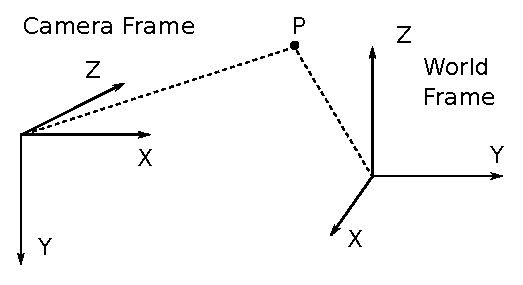
\includegraphics[width=.4\linewidth]{extrinsicparams.eps}
  \caption{Extrinsic parameters}
  \label{fig:pincam_ext}
\end{figure}

The camera's extrinsic parameters are its position and orientation in the 3D world. They are not constant, and change as the camera is displaced.\\

A camera can only take measurements relative to itself, so it makes sense to express the coordinates of 3D points in a coordinate frame relative to the camera. The camera's coordinate frame is defined as follows: the $Z$ direction is defined as pointing out of the camera, and the $X$ and $Y$ directions point towards the right and bottom of the image respectively (see figure \ref{fig:pincam_ext}). This works nicely with image coordinates, where $(0,0)$ is usually defined to be the top-left of the image.\\

However, because the camera will be moving around, points of the map have to be expressed in a reference coordinate system, constant and independent of the movement of the camera. The transformation between the reference coordinate system and the camera's coordinate system defines the camera's extrinsic parameters.\\

Let $p_w = (x_w, y_w, z_w)^T$ and $p_c = (x_c, y_c z_c)^T$ be the coordinates of point $p$ in a reference coordinate system and in the camera coordinate system respectively. Knowing the camera's position and orientation in the reference system, we can deduce the transformation to go from one coordinate system to the other:
\begin{equation}\label{eq:camframe}
  p_c = R \cdot p_w + t
\end{equation}
where $R$ is the rotation matrix between the two coordinate systems, and $t$ is the origin of the reference frame expressed in the camera coordinate system. Using homogenous coordinates, equation \ref{eq:camframe} can be rewritten as follows:
\begin{equation}\label{eq:camframe_bis}
  \begin{bmatrix}
     x_c \\
     y_c \\
     z_c
   \end{bmatrix}
     = [R|t]
   \begin{bmatrix}
      x_w \\
      y_w \\
      z_w \\
      1
   \end{bmatrix}
\end{equation}

The extrinsic parameters of the camera are its position, $t$, which has three degrees of freedom, as well as its orientation, represented by $R$, which also has three degrees of freedom. The orientation's degrees of freedom can be parametrized as three angles, for example the roll, pitch and yaw angles. It is possible to recover these angles from the rotation matrix, and vice versa. The task of localization will be to recover the camera's extrinsic parameters, and from these, the pose of the drone.

\subsubsection{Intrinsic Parameters}
\begin{figure}[H]
  \centering
  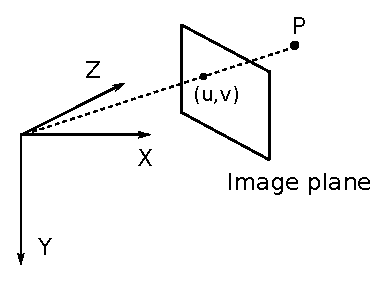
\includegraphics[width=.3\linewidth]{intrinsicparams.eps}
  \caption{Intrinsic parameters}
  \label{fig:pincam_int}
\end{figure}
Once we have the coordinates of point $p$ in the camera's system, we can project this point onto the image plane, using the camera's intrinsic parameters. These are the horizontal and vertical focal lengths $f_x$ and $f_y$, principal point coordinates $c_x$ and $c_y$ and skew factor $s$. From these, the image coordinates $u$ and $v$ can be recovered by projecting the three-dimensional coordinates as follows:
\begin{align}
  u &= \frac{f_xx_c + sy_c}{z_c} + c_x\\
  v &= \frac{f_yy_c}{z_c} + c_y
\end{align}
We can already see that our camera only gives information up to a scale factor, as multiplying all camera frame coordinates by a scalar gives the same image coordinates. The above equations can also we rewritten in matrix form, again using homogenous coordinates:
\begin{equation}
  z_c \begin{pmatrix} u\\v\\1 \end{pmatrix} =
  \begin{bmatrix}
  f_x & s   & c_x \\
  0   & f_y & c_y \\
  0   & 0   & 1
  \end{bmatrix} \begin{pmatrix} x_c\\y_c\\z_c \end{pmatrix}
\end{equation}
The matrix containing all intrinsic parameters of the camera is called the intrinsic matrix $K$:
\begin{equation}
  K = \begin{bmatrix}
  f_x & s   & c_x \\
  0   & f_y & c_y \\
  0   & 0   & 1
\end{bmatrix}
\end{equation}
The intrinsic parameters of the camera can be calculated from the output of the camera through a process called camera calibration. As their name implies, they are characteristics intrinsic to a camera, and do not change during operation, so they only need to be calculated once to be useable as known quantities.\\

Finally, the full projection from world coordinates to image coordinates can be performed as follows:
\begin{equation}
  z_c\begin{pmatrix} u\\v\\1\end{pmatrix} =
    K[R|t]\begin{pmatrix} x_w\\y_w\\z_w\\1\end{pmatrix}
\end{equation}
The projection matrix $P = K[R|t]$ gives the image coordinates up to a scale factor ($z_c$), but this can easily be resolved by normalizing the homogenous image coordinates so that the last coordinate is 1.

\subsection{Lens Distortion}
The pinhole camera model does not perfectly describe the projection of the world onto the camera's image, however, as it neglects lens distortion. Real cameras use lenses, and these lenses slightly deflect the light rays moving through them, so it is not accurate to consider that light travels in a straight line though a pinhole. This deflection causes distortion in the image. We consider two types of distortion: radial and tangential distortion. This distortion can be modeled using the Brown-Conrady distortion model (using a third order approximation for the radial distortion, and a second order approximation for the tangential distortion):
\begin{align}
	x_d &= x_u(1+k_1r^2+k_2r^4 + k_3r^6) + 2p_1x_uy_u + p_2(r^2 + 2x_u) \label{eq:dist1}\\
	y_d &= y_u(1+k_1r^2+k_2r^4 + k_3r^6) + 2p_2x_uy_u + p_1(r^2 + 2y_u) \label{eq:dist2}
\end{align}
Where $k_i$ and $p_i$ are the radial and tangential distortion coefficients respectively, $(x_d,y_d)$ is the distorted image point (where it is actually observed), $(x_u,y_u)$ is the undistorted image point (where it would be observed if there was no distortion), and $r = \sqrt{(x_u - x_c)^2 + (y_u - y_c)^2}$ is the distance between the undistorted point, and the image center $(x_c, y_c)$.  \\
If we know $(k_1,k_2,k_3,p_1,p_2)$, we can invert equations \ref{eq:dist1} and \ref{eq:dist2} to obtain the undistorted points. \cite{opencvcamcalib}

\subsection{Camera calibration}
Both the distortion coefficients and the camera matrix (consisting of the focal lengths, principal point, and skew factor) are intrinsic to the camera. It would be useful to know them once and for all, as they do not change during operation.\\

The process of camera calibration refers to the estimation of the distortion coefficients and camera matrix. It is typically done by looking at checkerboards placed at various points in the camera's field of view. The distortion coefficients are optimized such that the corners on the checkerboards appear on straight lines. The fact that the points of the checkerboard are part of the same plane, and that they form squares is used to estimate the camera's intrinsic parameters. There is a convenient ROS node called \texttt{camera\_calibration} that does this.\\

To be able to use the pinhole camera model in all our algorithms, we will use another convenient ROS node called \texttt{image\_proc} that takes a stream of distorted images as input, and uses the distortion coefficients that were previously estimated to produce a stream of undistorted images as output.

\section{Scale-space representation}
One of the problems when trying to recognize points from a variety of viewpoints, is that depending on the distance between the point and the camera, the point can have many different sizes in the image. The scale-space representation is an attempt to solve this problem. An image can be represented as a two variable function $f(x,y)$, where the value of $f$ is the intensity of the pixel at location $(x,y)$. The scale-space representation of $f$ is a family of signals obtained by convoluting the original signal with a Gaussian filter $g$: $L(x,y;\sigma) = g(x,y;\sigma) \star f(x,y)$. For different values of the parameter $\sigma$ (the scale), the result is a blurred image where finer and finer details are indistinguishable. When $\sigma=0$, the Gaussian becomes an impulse function and the result of the convolution is the original image. The scale-space representation of an image, $L(x,y,\sigma)$ can be seen as a three dimensional image, made by stacking images obtained by blurring the source image more and more. By working on the scale-space representation of images, we ensure that our methods are scale invariant. \cite{scalespace}\\

To illustrate this with an example, we look at figure \ref{fig:scalespace}. Images \ref{fig:scalespace_faraway} and \ref{fig:scalespace_closeby} have been observed and we would like to match them. Zooming in on image \ref{fig:scalespace_faraway} gives \ref{fig:scalespace_faraway_zoomedin}, but this image is quite different from \ref{fig:scalespace_closeby}. If we look at the scale-space representation of \ref{fig:scalespace_closeby} we might find a match at higher scales, when the image becomes blurred to look like image \ref{fig:scalespace_closeby_blurred}. Note that we are matching individual keypoints, which are usually smaller than this image (the corners of this image could each be keypoints).

\begin{figure}[H]
\centering
\begin{subfigure}{.4\textwidth}
  \centering
  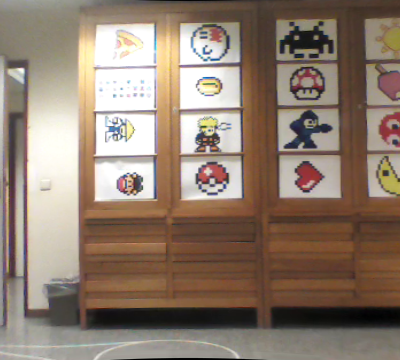
\includegraphics[width=.9\linewidth]{scalespace_faraway.png}
  \caption{View from far away.}
  \label{fig:scalespace_faraway}
\end{subfigure}%
\begin{subfigure}{.4\textwidth}
  \centering
  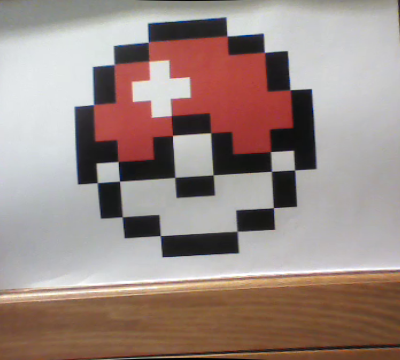
\includegraphics[width=.9\linewidth]{scalespace_closeby.png}
  \caption{View from close by.}
  \label{fig:scalespace_closeby}
\end{subfigure} \\
\begin{subfigure}{.4\textwidth}
  \centering
  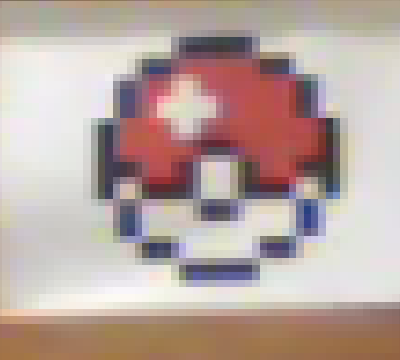
\includegraphics[width=.9\linewidth]{scalespace_faraway_zoomedin.png}
  \caption{From far away, zoomed in.}
  \label{fig:scalespace_faraway_zoomedin}
\end{subfigure}%
\begin{subfigure}{.4\textwidth}
  \centering
  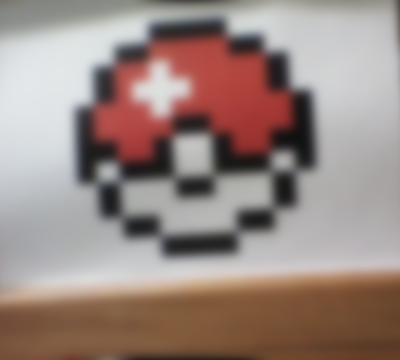
\includegraphics[width=.9\linewidth]{scalespace_closeby_blurred.png}
  \caption{From close by, filtered by a Gaussian.}
  \label{fig:scalespace_closeby_blurred}
\end{subfigure}
\caption{Usefulness of the scale-space representation.}
\label{fig:scalespace}
\end{figure}

\section{SURF Keypoint Detector}
The SURF detector uses the determinant of the Hessian matrix to measure local change around points. The Hessian matrix is defined as follows:
\begin{equation}
  \mathcal{H}(\bf{x},\sigma) =  \begin{bmatrix}
  L_{xx}(\bf{x},\sigma) & L_{xy}(\bf{x},\sigma)\\
  L_{xy}(\bf{x},\sigma) & L_{yy}(\bf{x},\sigma)
\end{bmatrix}
\end{equation}
where $L_{xx}$, $L_{xy}$ and $L_{yy}$ are the convolution of the image with the second order derivatives of the Gaussian $g(\bf{x};\sigma)$. The creators of SURF decided to approximate the second order Gaussian derivatives with box filters. This decision stemmed from the fact that even though Gaussian filters are optimal, they are already modified quite heavily, as they have to be discretized and cropped, and the result of the convolution is then resampled. The big advantage of using square filters is that they can be evaluated very quickly by using integral images. To obtain a scale-space representation, the SURF method uses box filters of different sizes: for example, a 9x9 filter, approximates a Gaussian with parameter $\sigma = 1.2$, with larger filters corresponding to bigger values of $\sigma$. Local maxima on 3x3x3 neighborhoods of the scale-space representation are then taken as points of interest.\\

Finally, so that the detected keypoints are rotationally invariant, we need to assign an orientation to each keypoint that can be recognized from subsequent viewpoints. To do this, the SURF method computes the response to vertical and horizontal Haar wavelets in a circular neighborhood of radius $6s$ around the detected points, $s$ being the scale at which that point was detected. The Haar wavelets are rectangle shaped, so their response can also be computed efficiently using integral images. The responses are plotted in a plane, where the abscissa is the horizontal response, and the ordinate is the vertical response. The responses are summed within a sliding orientation window, giving an orientation vector for each position of the sliding window. The orientation vector with the largest norm is taken to be the orientation of the keypoint.
\cite{surf}

\section{SIFT Keypoint Descriptor}
\begin{figure}[H]
  \centering
  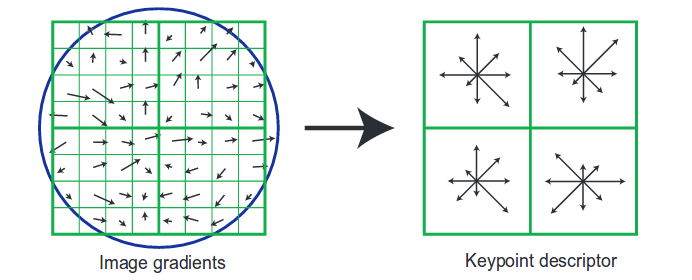
\includegraphics[width=\textwidth]{siftdescriptor.png}
    \caption{Illustration of a SIFT descriptor. Each subregion containing 4x4 points defines a histogram with 8 bins. Note that SIFT uses 4x4 subregions, not 2x2 like in this illustration. \cite{sift2}}
    \label{fig:siftdescriptor}
\end{figure}
To create a SIFT descriptor, a 16x16 square region is taken around the keypoint. This region is rotated and scaled according to the orientation and scale of the detected keypoint. The 16x16 region is subdivided into 16 4x4 subregions. In each subregion, a histogram of local gradients is computed and quantized into 8 bins. The magnitudes of these histograms form the descriptor. Figure \ref{fig:siftdescriptor} shows an illustration of the histograms. As there are 16 histograms of 8 bins each, the total length of the descriptor vector is 128. \cite{sift}

\subsection{Limitations}
The dimension of SIFT descriptors is 128, which is quite large. Having such a large dimension has the advantage of allowing the descriptors to be highly discriminative, even with many different keypoints, but the disadvantage of requiring more space to be saved, and to slow down the matching algorithms that will be used later on.\\

Another limitation is that the points detected are points of the image with a high intensity gradient. These points are often corners, with two distinctive regions, one inside and one outside the corner. The descriptor depends on the gradients of the image, which depend on both these regions. To be able to recognize the keypoints, the descriptors have to be similar independently of the viewpoint of the keypoint. This is the case when both regions of the corner are part of the same plane, like in the case of a 2D drawing, but it is not the case when the inside of the corner is some object, and the outside is the background, as the background can change depending on the viewpoint. For example, figure \ref{fig:siftlimit} shows the same point seen from two different angles, where the descriptor would be quite different, because there is a different background
\begin{figure}[H]
\centering
\begin{subfigure}{.4\textwidth}
  \centering
  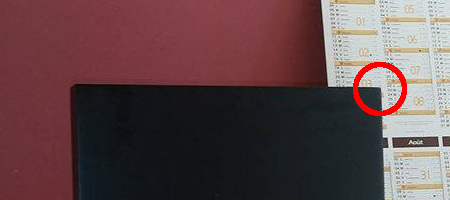
\includegraphics[width=.9\linewidth]{siftlimit1.png}
\end{subfigure}%
\begin{subfigure}{.4\textwidth}
  \centering
  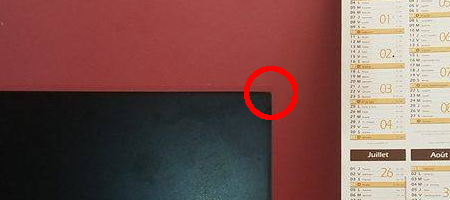
\includegraphics[width=.9\linewidth]{siftlimit2.png}
\end{subfigure} \\
\caption{Two views of a same point, with a different background.}
\label{fig:siftlimit}
\end{figure}

\section{Keypoint Tracking}
Because the above algorithm to extract a descriptor of a keypoint is quite slow (it takes approximately \SI{413}{\milli\second} to extract all descriptors from a new image, see table \ref{tab:cvtime}), it is not practical to run these algorithms on each new image, as this would greatly reduce the frame rate. For this reason, another, faster alternative has been found : keypoint tracking. This method finds keypoints by looking for keypoints that were observed in the previous image, and assuming that their displacement inside the image was small. \\

The algorithm used for this keypoint tracking is called the pyramidal Lucas-Kanade method \cite{pyramidallucaskanade}. This method assumes that the movement between successive frames is small and can be approximated by an affine transformation in local regions. It uses small dense pixel regions to estimate the movement of a keypoint between successive frames. The method was explained more in detail in last year's master thesis \cite{jacquesleclere}.\\

Keypoint tracking has the advantage of being much faster than detecting new keypoints, especially because the descriptor of each tracked keypoint is already known and does not have to be extracted again at each frame. The main drawback of this method is that it does not allow to detect any new keypoints, as all tracked keypoints have to be present in the previous frame.

\section{Detection and Tracking hybrid}

In the previous years, detection and tracking were used alternatively: each new frame was populated with keypoints using one of the two methods. As long as there were enough keypoints in the preceding frame, tracking was used on all these keypoints with no detection of new keypoints. While tracking is used, the number of keypoints in each successive frame is non-increasing, as each keypoint can either be lost or tracked, and when the number of keypoints in the frame fell below some threshold, keypoint detection was used to populate the next frame with new keypoints.\\

When the detection method is used, all previous keypoints are discarded, and keypoints are detected on the entire image. The reason for this choice was that detection was too slow to be used on each frame, but necessary to find new keypoints, and that if detection and tracking were used simultaneously, keypoints that are already being tracked would be re-detected, which would result in duplicate keypoints in the same frame. However, this method is suboptimal, because every time detection is used, all currently tracked keypoints are lost and have to be re-detected. It also causes quite an inconsistent frame rate.\\

\begin{figure}[H]
  \centering
  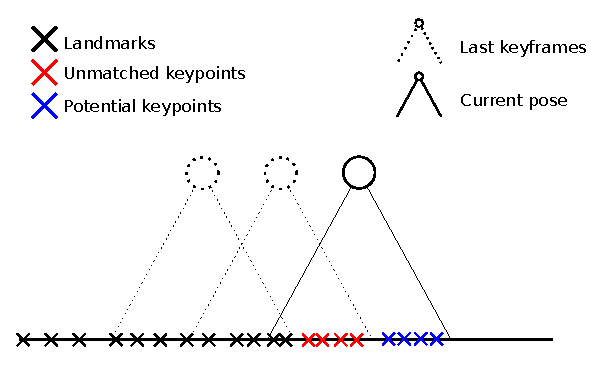
\includegraphics{keyframe_landmark_illustration.eps}
  \caption{Delay between first observation of a keypoint, and mapping of this keypoint.}
  \label{fig:delay}
\end{figure}

In addition to being suboptimal, this method has a few drawbacks that make it hard to use for this project. As we will see later, at least two views of a single keypoint from different keyframes are required to estimate the 3D position of the corresponding landmark. Figure \ref{fig:delay} is an illustration of this problem, in a one dimensional world. When a keypoint is seen for the first time and saved in a keyframe, it becomes an unmatched keypoint (red cross), and its 3D location is unknown. It has to be observed from a second keyframe in order to become a landmark (black cross), with an estimated 3D position. Only then can it be used as a reference to localize the drone.\\

On figure \ref{fig:delay}, if the drone creates a new keyframe at its current position, the unmatched keypoints can become landmarks, and the potential keypoints (blue crosses) become new unmatched keypoints. If we had only used tracking since the last keyframe, however, we would not have detected those potential keypoints. As a result, when the drone continues advancing it would not have any unmatched keypoints from the previous keyframe, and it would not be able to add any landmarks to the map. The difficulty lies in the fact that each time we create a new keyframe, we ideally need to see:

\begin{enumerate}
\item Enough already mapped landmarks to accurately estimate the position of the new keyframe
\item Unmatched keypoints from previous keyframes so that we can put them into the map to allow further exploration
\item New, previously unobserved keypoints to ensure long-term viability (these points will be the unmatched keypoints of the next keyframe)
\end{enumerate}

The need for these three ingredients means that keyframes have to be created more frequently than when we are mapping keypoints from single observations. In many cases, there are enough common keypoints between successive keyframes so that the old method did not require detection at any moment between the two keyframes. As a result, all keypoints of the most recent keyframe would already have been observed before. This means that they can be added to the map, but it seriously harms possible future exploration, as the third element of the above list is missing, so it won't be able to create any new landmarks when the next keyframe is created. Simply decreasing the threshold at which we used detection instead of tracking was not a good solution as it resulted in many more slow detection steps.\\

To solve this problem, a new technique had to be found. It is clear that we need new, unmatched keypoints in each keyframe, and these points cannot be tracked from previous images, so they have to be detected. However, keypoint detection takes so much time it's prohibitive to do it on each image. We noticed that the vast majority of keypoints that are lost during tracking are lost because they are moved out of the field of vision, so they leave the image from the sides. Similarly, new potential keypoints enter the field of view from the sides, so after some displacements, there will often be sections of the image with many keypoints (parts of the scene that were observed continuously since the last full keypoint detection), and sections of the image with no keypoints (parts of the scene that were not in the field of view when the last full detection took place). Our solution is to treat the part of the image with no keypoints as if it was a separate image, and do keypoint detection on that part, while keeping the part of the image with keypoints, and tracking its keypoints. This is illustrated on figure \ref{fig:trackdetecthybrid}.

\begin{figure}[H]
\centering
\begin{subfigure}{.33\textwidth}
  \centering
  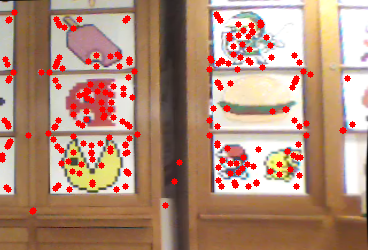
\includegraphics[width=.9\linewidth]{track_detect_hybrid_start.png}
  \caption{Initial frame}
  \label{fig:trackdetecthybrid_a}
\end{subfigure}%
\begin{subfigure}{.33\textwidth}
  \centering
  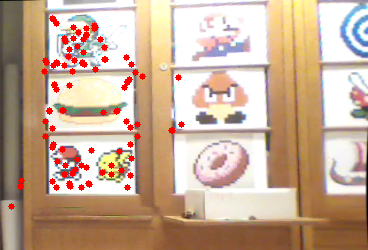
\includegraphics[width=.9\linewidth]{track_detect_hybrid_mid.png}
  \caption{After displacement and tracking}
  \label{fig:trackdetecthybrid_b}
\end{subfigure}
\begin{subfigure}{.33\textwidth}
  \centering
  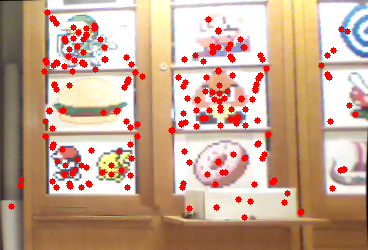
\includegraphics[width=.9\linewidth]{track_detect_hybrid_end.png}
  \caption{After detection}
  \label{fig:trackdetecthybrid_c}
\end{subfigure}
\caption{Illustration of the hybrid between tracking and detection.}
\label{fig:trackdetecthybrid}
\end{figure}

We can see on table \ref{tab:cvtime} that our hybrid method takes about \SI{55}{\milli\second} per image. This is the time for both the tracking of the keypoints of the previous image, and detection and description of keypoints on the sides. Ideally, we would like this time to be below \SI{33}{\milli\second}, because our front camera has a rate of 30 FPS, so it sends an image every \SI{33}{\milli\second}. However, we do not need to use our hybrid at every new image, only when a significant part of the sides of the image contains no points from tracking. The rest of the time, we can use pure tracking, which runs in \SI{6}{\milli\second}. In the end we are alternating between tracking and our hybrid method, instead of between tracking and full detection. The end result is that we are more regular, both in the number of keypoints of any given frame, and in the computation time required per frame.

\begin{table}[H]
  \centering
  \small\addtolength{\tabcolsep}{-2pt}
  \sisetup{round-mode=places, round-precision = 3}
  \begin{tabular}{ @{} l @{\hspace{10mm}}     S[table-format=3.0] @{}  }
    \toprule
    Task & \multicolumn{1}{l}{Time per Frame [\si{second}[]}  \\
    \midrule
    Keypoint detection   & \num{0.032} \\
    Keypoint description & \num{0.413} \\
    Keypoint tracking    & \num{0.006} \\
    Hybrid               & \num{0.055} \\
    \bottomrule
  \end{tabular}
  \caption{Timings for the different tasks. The time for the hybrid method includes tracking, detection, and description.}
  \label{tab:cvtime}
\end{table}
\newpage
\section{Keypoint Matching}
The final computer vision task is keypoint matching. After keypoints from multiple viewpoints are saved, we need to know which observations correspond to the same point. This is needed when a keyframe is added to the map, because we need keypoint matches to place landmarks in the map, and also when trying to match an image with the map to localize the drone. We will compare the descriptors of the keypoints to determine which ones are similar enough to represent the same point. The Euclidean distance is a good metric of how different the descriptors are, because they are vectors of floating point numbers (if we were working with binary descriptors, like in the case of BRIEF, we should use the Hamming distance instead).\\

When matching a query image with a reference image, we find the nearest descriptor of the reference image for each descriptor of the query image. For each pair, we then determine if they are close enough to be considered a match. Finding the exact nearest neighbor would take $O(n*m)$ time for an exhaustive search, where $n$ and $m$ are respectively the number of keypoints in the query and in the reference images. A search with a k-d tree runs in $O(n\log(m))$ time, but suffers from the curse of dimensionality, so in high dimensional spaces it is not always faster than an exhaustive search in practice.\\

To overcome these problems, we only look for an approximate nearest neighbor. There exist many different approximate nearest neighbor methods, one of the most famous for high dimensional search is the best-bin first method, which was recommended by the creators of SIFT. It is based on a k-d tree and finds the nearest neighbor in most cases, and a very close neighbor the rest of the time. Other, better approximate nearest neighbor methods have since been invented, so to marginalize the choice of an approximate nearest neighbor algorithm, we use the implementation of a FLANN matcher of OpenCV for the nearest neighbor computation. FLANN stands for Fast Library for Approximate Nearest Neighbors. It contains many state-of-the-art nearest neighbors algorithms and automatically chooses the most appropriate one depending on the data. It is quite fast: to find amongst $666$ keypoints of a keyframe the closest match for each of $502$ keypoints of another keyframe, it took approximately \SI{21}{\milli\second}.

\section{Summary}
In the code, the computer vision node serves as an intermediary between the output of the camera and the input of the localization and mapping nodes. It transforms each image into a list of keypoints, each with their 2-dimension location on the image plane, and 128-dimension descriptor. To do this, it first undistorts the image, using distortion coefficients estimated in advance, then either tracks keypoints from the previous frame, and detects descriptors at the edges of the frame, or discards all keypoints of the previous frame and detects keypoints on the entire image. In both cases, descriptors for the newly detected keypoints are then extracted. Later, the localization and the mapping nodes can use keypoint matching to find keypoints in different frames that correspond to the same landmark.\\

In this part, we kept using SIFT descriptors and a SURF detector, as was implemented last year, but the OpenCV library contains procedures for working with many other types of descriptors and detectors, which were not tested this year. In future work on this project, it might be interesting to test using other types of keypoints, such as ORB, as the tests leading to the choice for the current SIFT/SURF combination were made before the current 3D framework existed.\\
Figure \ref{fig:cvflowchart} summarizes the computer vision part of the code in the form of a flowchart.

\begin{figure}[H]
\centering
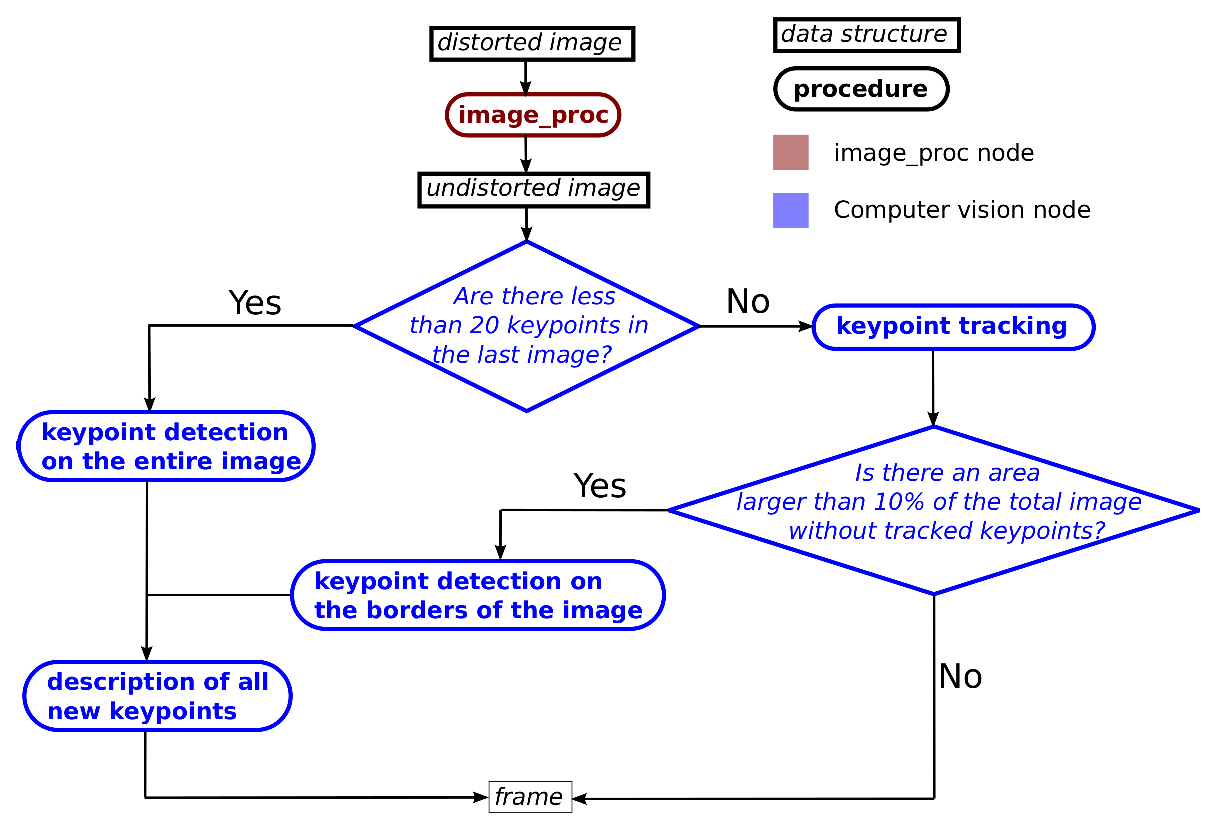
\includegraphics[width=\linewidth]{cvflowchart.eps}
\caption{Flowchart of computer vision node}
\label{fig:cvflowchart}
\end{figure}
